\section{Feature Extraction in Audio}

To extract features from audio, we use the MFCC
(Mel-Frequency Cepstral Coefficients) technique and
spectrograms to visualize the audio. The audio feature
extraction process will include steps such as Pre-emphasis,
Windowing, DFT (Discrete Fourier Transform), etc.\cite{hossan2011novel}, as follows:

\vspace{-1em}
\begin{figure}[H]
    \centering
    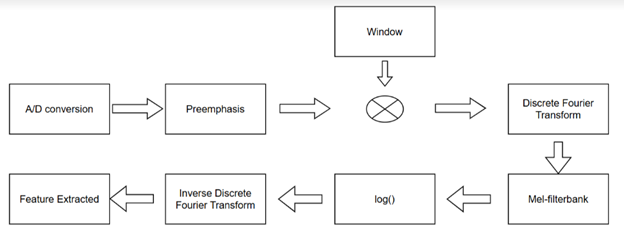
\includegraphics[width=0.47\textwidth]{Audio-Feature-Extraction-Steps.png}
    \caption{Audio Feature Extraction Steps}
    \label{fig:audio-feature-extraction-steps}
\end{figure}
\vspace{-1em}

\subsection{Pre-emphasis}

Pre-emphasis is a signal processing technique commonly used
in the context of audio and speech processing. It is applied
to the input audio signal before proceeding with subsequent
processing steps, such as calculations in MFCC. The purpose of
pre-emphasis is to emphasize higher frequencies in the audio
signal, which often have lower energy compared to lower
frequencies. This helps improve the Signal-to-Noise Ratio
(SNR) and enhance the clarity of speech or other audio
signals, especially in subsequent processing steps.

Mathematically, pre-emphasis is performed as a high-pass
filter between high frequencies compared to lower frequencies.
Typically, it is performed using a first-order FIR
(Finite Impulse Response) filter with a simple equation:

\vspace{-1em}
\begin{equation}
    y[n] = x[n] - \alpha \cdot x[n-1]
\end{equation}
\vspace{-1em}

Where:
\begin{itemize}
    \item $y(n)$: Output signal after pre-emphasis.
    \item $x(n)$: Input audio signal.
    \item $\alpha$: Pre-emphasis coefficient in the range from 0.9 to 0.97.
\end{itemize}

This filter operates by subtracting a scaled version of the
previous sample from the current sample, effectively
amplifying high-frequency components and attenuating
low-frequency components. This compensates for the spectral
tilt typically observed in speech and other audio signals,
resulting in a flatter frequency response and improved
intelligibility.

\subsection{Windows}

Instead of performing a Fourier transform on the entire long
audio segment, we slide a window along the signal to extract
smaller audio segments and then apply the DFT to each of these
segments. However, each window should be divided into three
parts: pre-emphasis, the current segment, and post-emphasis.
This helps avoid losing information from each extracted audio
segment. Each window also needs to overlap to better preserve
information; typically, windows overlap by about $10ms$.

\vspace{-1em}
\begin{figure}[H]
    \centering
    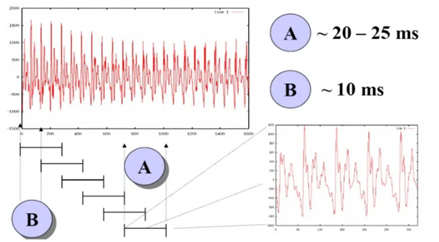
\includegraphics[width=0.47\textwidth]{Windowing-Technique-for-Audio-Signals.png}
    \caption{Windowing Technique for Audio Signals}
    \label{fig:windowing-technique-for-audio-signals}
\end{figure}
\vspace{-1em}

\subsection{Discrete Fourier Transform and Spectrograms:}

Using the Fourier transform, a time-domain signal can be
transformed into its frequency-domain representation. This
transformation provides information about the frequency
content of the signal, including both the frequencies present
and their corresponding magnitudes.

\vspace{-1em}
\begin{figure}[H]
    \centering
    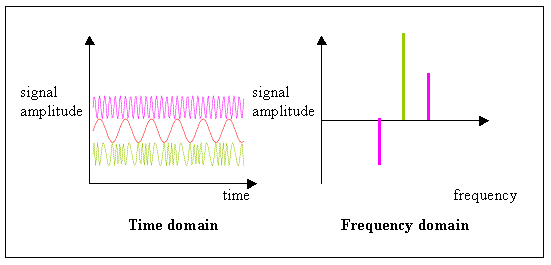
\includegraphics[width=0.47\textwidth]{Fourier-Transform-of-a-Sound-Signal.png}
    \caption{Fourier Transform of a Sound Signal \cite{technical_editor_2017}.}
    \label{fig:fourier-transform-of-a-sound-signal}
\end{figure}
\vspace{-1em}

The Fourier transform provides a frequency-domain
representation of the signal, resulting in a magnitude
spectrum. However, this transformation inherently loses time
localization information, making it impossible to determine
the temporal occurrence of specific frequency components. To
overcome this limitation, a time-frequency representation is
required, which is provided by the spectrogram. In a
spectrogram, the abscissa represents time, the ordinate
represents frequency, and the color intensity represents the
magnitude of the spectral components. Higher color intensity
corresponds to higher magnitudes (stronger frequency components).

\vspace{-1em}
\begin{figure}[H]
    \centering
    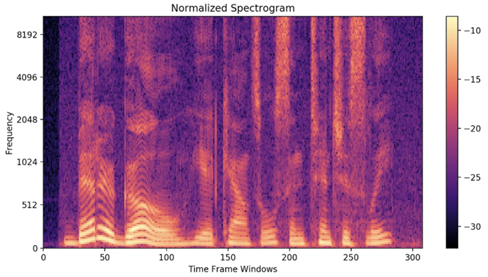
\includegraphics[width=0.47\textwidth]{Spectrogram-after-applying-Fourier-transform.png}
    \caption{Frequency Spectrum after Fourier Transform}
    \label{fig:spectrogram-after-applying-fourier-transform}
\end{figure}
\vspace{-1em}

The Discrete Fourier Transform (DFT) is mathematically defined
as:

\begin{equation}
    X[k] = \sum_{n=0}^{N-1} x[n] \cdot e^{-i \frac{2\pi}{N}kn}
\end{equation}

Where:
\begin{itemize}
    \item $X[k]$: Represents the complex-valued amplitude of the
          $k^{th}$ frequency component in the frequency domain. It's
          often referred to as the $k^{th}$ "frequency bin" or "spectral
          component".

    \item $x[n]$: Denotes the $n^{th}$ sample of the input signal
          in the time domain.

    \item $N$: Is the total number of samples in the input
          signal being analyzed.

    \item $k$: Is the frequency index, taking integer values
          from $0$ to $N-1$. These values correspond to discrete
          frequencies ranging from $0$ Hz to $\frac{(N-1)}{N}$ times the
          sampling frequency. The maximum frequency (when $k = \frac{N}{2}$
          for even $N$) is known as the Nyquist frequency.

    \item $j$: Represents the imaginary unit, defined as $\sqrt{-1}$.
          This indicates that $X[k]$ is a complex number with both
          real and imaginary parts (or magnitude and phase).

    \item $n$: Is the sample index in the time domain,
          iterating from $0$ to $N-1$ within the summation.

    \item $k$: Is the frequency index, indicating which
          frequency component is being computed.

\end{itemize}

In essence, the DFT is a crucial step in MFCC extraction,
transforming the time-domain input signal into its frequency-
domain representation. This decomposition into individual
frequency components facilitates the creation of a spectrogram,
a visual representation of the signal's frequency content over
time. This representation simplifies subsequent machine
learning tasks by providing relevant features in a more
manageable and informative form.

\subsection{Mel-filterbank}
The human auditory system exhibits a non-linear frequency
response, demonstrating greater sensitivity to changes in
lower frequencies and reduced sensitivity to changes in higher
frequencies. The Mel filterbank is designed to model this
perceptual non-linearity, providing a perceptually relevant
representation of the audio signal.

The Mel scale is a psychoacoustic scale of perceived pitch
based on human auditory perception. It is characterized by a
non-linear relationship with linear frequency (Hz), with a
greater emphasis on the lower frequency region.

The conversion from linear frequency (Hertz) to Mel frequency
is often done using a formula like this:

\begin{equation}
    f_{mel} = 2595 \cdot \log\left(1 + \frac{f}{500}\right)
\end{equation}

The Mel filterbank operates on the power spectrum of an audio
signal. The power spectrum provides a representation of the
signal's energy distribution across discrete frequency bins.
Each triangular filter of the Mel filterbank is convolved with
the power spectrum, yielding a series of filter bank outputs.

\vspace{-1em}
\begin{figure}[H]
    \centering
    \includegraphics[width=0.47\textwidth]{Mel-Filterbank.png}
    \caption{Mel-filterbank}
    \label{fig:mel-filterbank}
\end{figure}
\vspace{-1em}

The filter bank outputs represent an approximation of the
signal's energy distribution across various frequency bins,
with higher output magnitudes signifying greater energy
concentration within the corresponding frequency bins. These
outputs capture the signal's energy distribution across
different frequency bands in a perceptually significant
manner.

Squaring the magnitude spectrum obtained from the DFT,
followed by the application of a Mel-scale filterbank across
the frequency axis, results in each filter output representing
the integrated energy within its corresponding Mel-scaled
frequency band. The resulting representation is referred to as
the Mel-scale spectrum.

\vspace{-1em}
\begin{figure}[H]
    \centering
    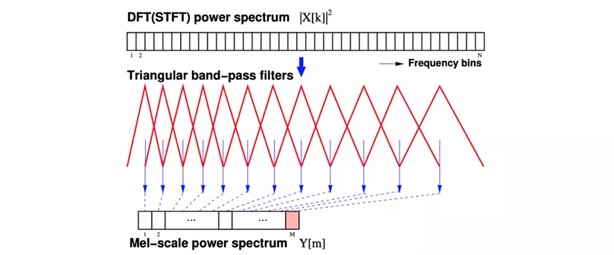
\includegraphics[width=0.47\textwidth]{Mel-Scale-Conversion-of-the-DFT-Spectrum.png}
    \caption{Mel-Scale Conversion of the DFT Spectrum \cite{nacem2020subspace}}
    \label{fig:mel-scale-conversion-of-the-dft-spectrum}
\end{figure}
\vspace{-1em}

\subsection{log()}

The role of the logarithm function in calculating
Mel-Frequency Cepstral Coefficients (MFCCs) is to compress
the dynamic range of the filter output values. Logarithmic
compression helps make the MFCC representation more robust to
variations in signal intensity and enhances its discriminative
ability.

Assuming an input signal $x$ with impulse response $h$, the
resulting audio spectrum in terms of sound intensity is:

\begin{equation}
    |Y(w)| = |X(w)| \cdot |H(w)|
\end{equation}

After applying the logarithm, we obtain:

\begin{equation}
    \log|Y(w)| = \log|X(w)| + \log|H(w)|
\end{equation}

\subsection{Discrete Cosine Transform (DCT)}

The Discrete Cosine Transform (DCT) constitutes the final
stage of MFCC feature extraction. The fundamental concept
behind the DCT is analogous to that of the Inverse Discrete
Fourier Transform (IDFT). Following MFCC feature extraction,
a transformation from the frequency domain to the time domain
is conducted. The MFCC representation typically utilizes the
first $12$ coefficients obtained from the IDFT, augmented with
the energy term, as its characteristic features.

\vspace{-1em}
\begin{figure}[H]
    \centering
    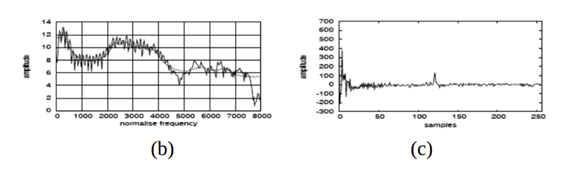
\includegraphics[width=0.47\textwidth]{Time-Domain-Signal-Reconstructed-from-IDFT.png}
    \caption{Time-Domain Signal Reconstructed from IDFT}
    \label{fig:time-domain-signal-reconstructed-from-idft}
\end{figure}
\vspace{-1em}

The dominant frequency observed at the center of
\autoref{fig:time-domain-signal-reconstructed-from-idft}c
corresponds to $F_0$, the fundamental frequency of the acoustic 
signal. $F_0$ serves as a distinguishing characteristic of an 
individual's voice pitch. The leftmost region of the figure 
represents phonetic information associated with the formants 
$F_1$, $F_2$, etc. Within the context of sound classification, the 
fundamental frequency $F_0$ and the formant frequencies $F_1$, $F_2$, $F3$, 
and so forth, constitute important features for speaker 
characterization.

\subsection{Dynamic features}

The MFCC process results in $39$ features, of which the first $12$ 
are obtained by applying the DCT (Discrete Cosine Transform) 
to the $\log$ Mel spectrum. The $13^{th}$ feature is the energy of 
each time frame. The remaining $26$ features are divided into 
two sets of $13$ features each. The first set of $13$ features is 
used to calculate the first-order derivatives (delta 
coefficients), and the last $13$ features are used to calculate 
the second-order derivatives (delta-delta coefficients) at 
time $x$:

\begin{equation}
    f'(x) = \frac{f(x + \Delta t) - f(x - \Delta t)}{2\Delta t}
\end{equation}

\begin{equation}
    f''(x) = \frac{f'(x + \Delta t) - f'(x - \Delta t)}{2\Delta t}
\end{equation}

By calculating the first-order and second-order derivatives 
of MFCCs or other feature vectors, the temporal dynamics and 
variations within the signal can be captured, providing 
additional information that can be useful for tasks such as 
speech recognition, speaker recognition, and emotion 
recognition. These derivatives can be concatenated with the 
original feature vectors to create extended feature 
representations to improve performance in such tasks.
